%!TEX root = ../thesis.tex
\chapter{Introduction}  % Main chapter title
\label{cha:introduction} 

%----------------------------------------------------------------------------------------
%	SECTION 1
%----------------------------------------------------------------------------------------

\section{Main Section 1}


MR relation ship image arXiv:1506.05097 \citet{chen_probabilistic_2016}

\begin{figure}
    \centering
    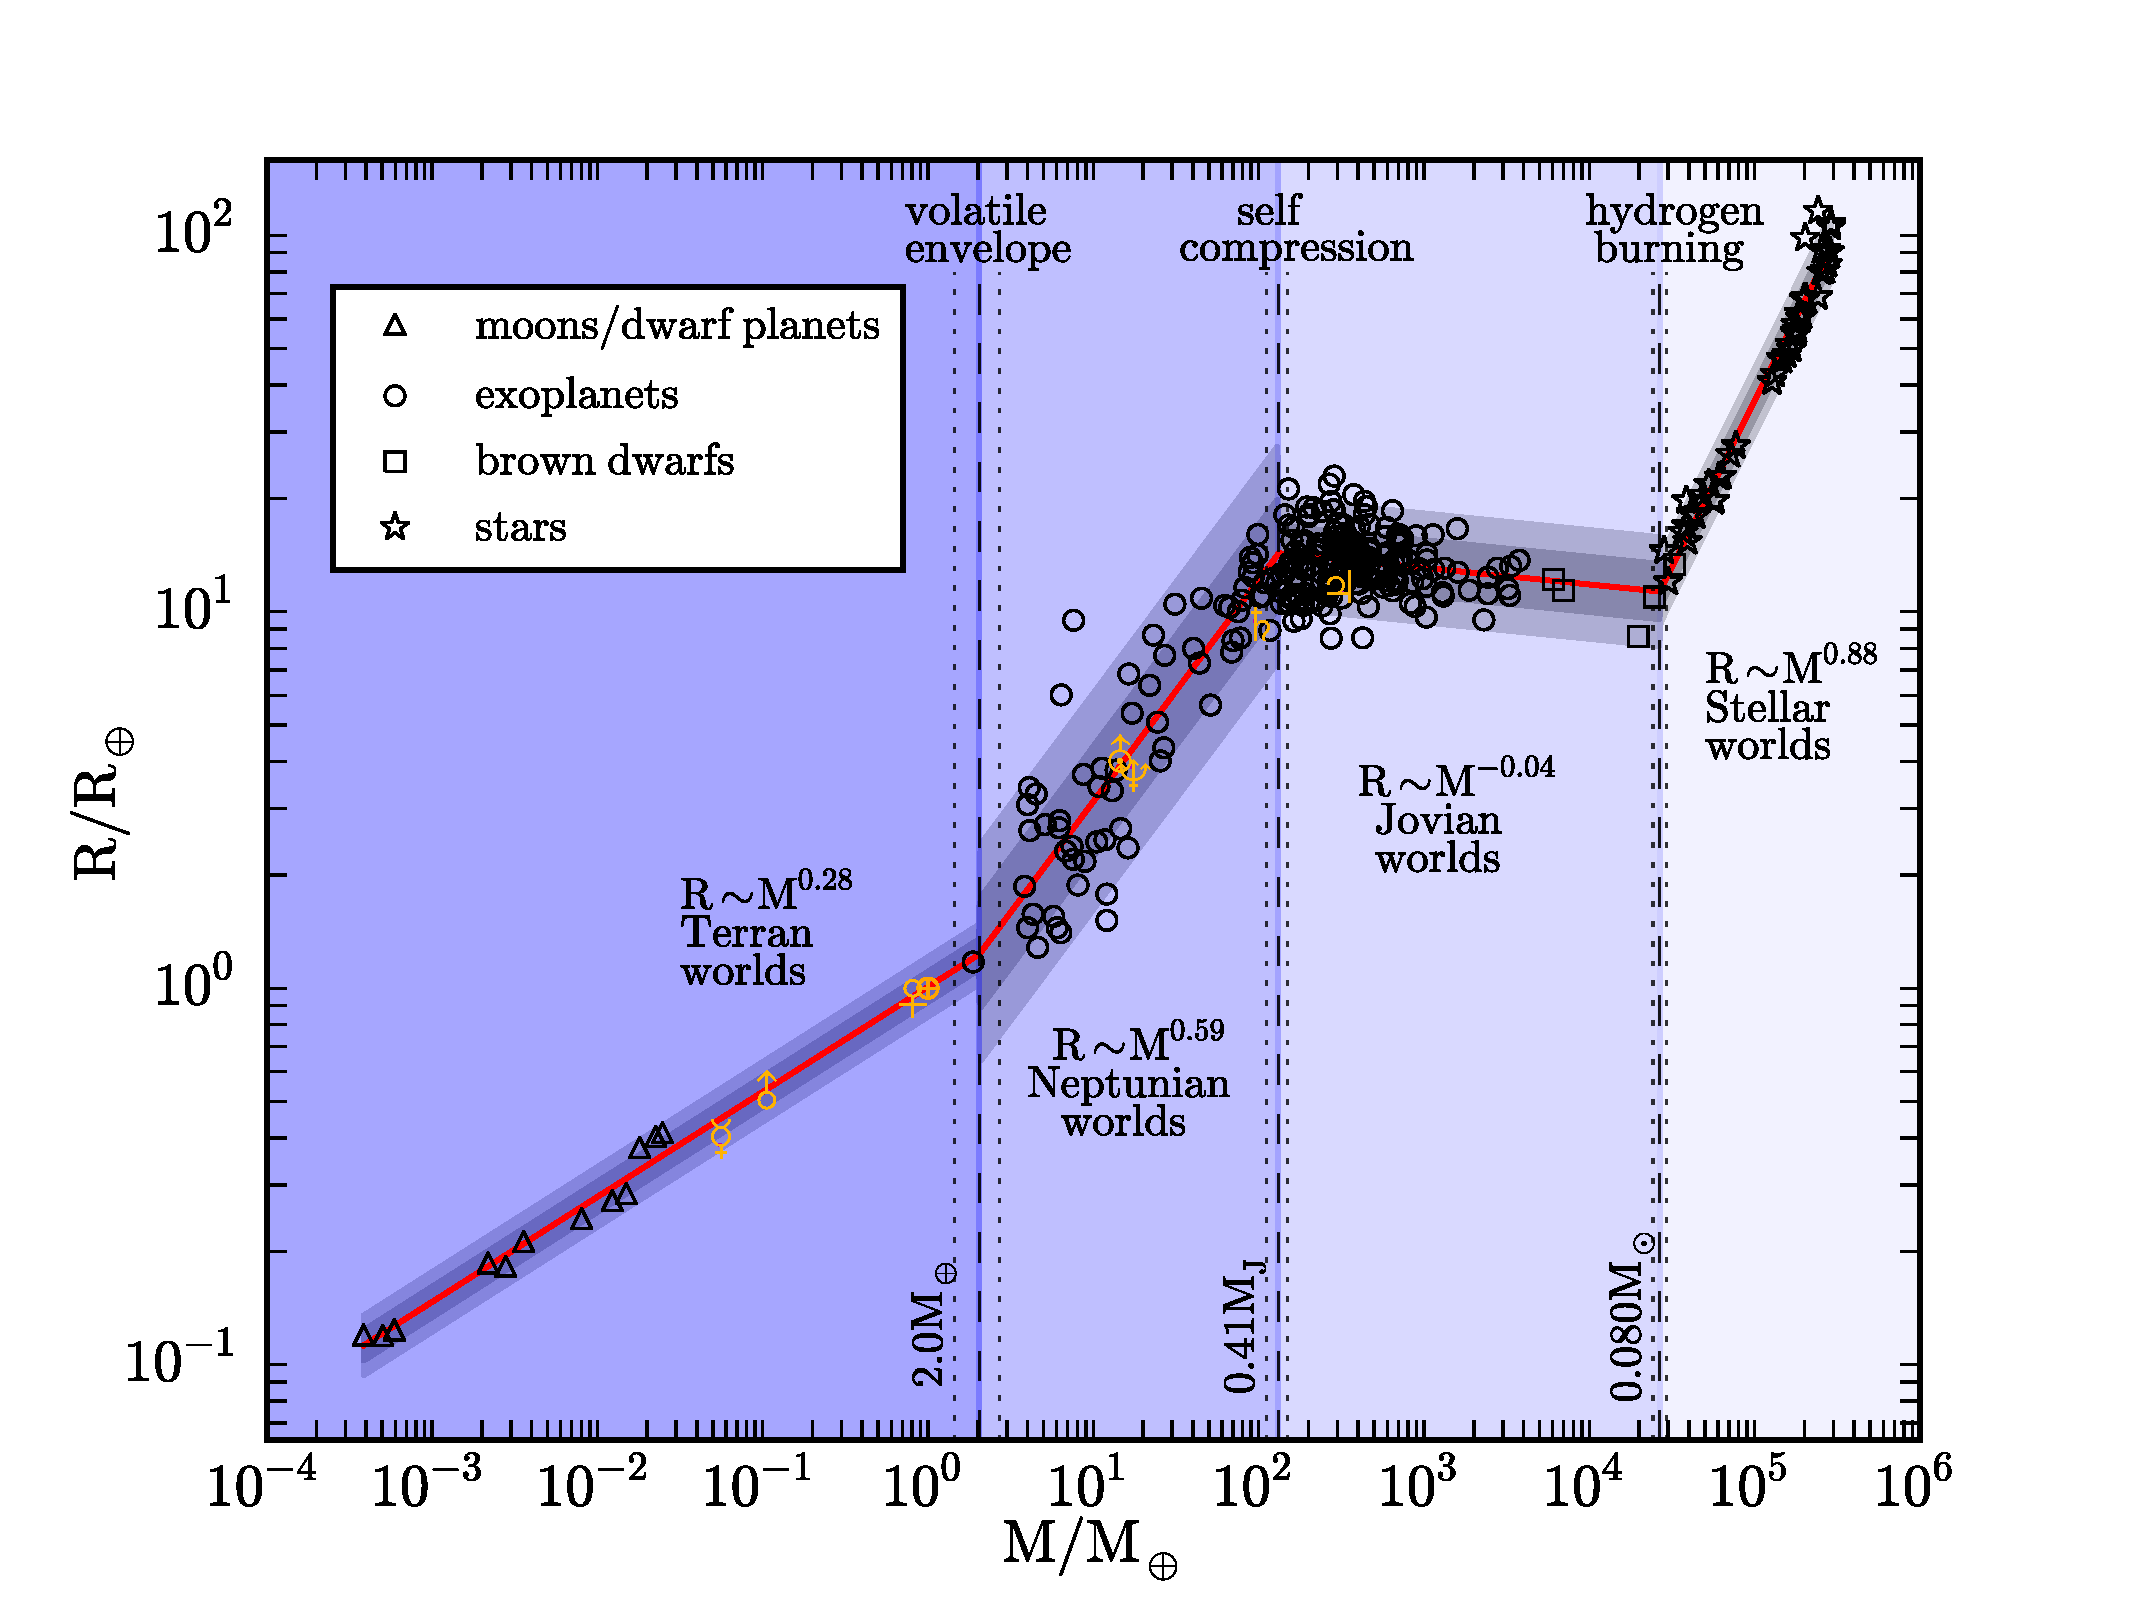
\includegraphics[width=0.7\linewidth]{./figures/introduction/plt_overlay_add.pdf}
    \caption{ M-R relationship \citet{chen_probabilistic_2016}}
    \label{fig:pltoverlayadd}
\end{figure}

Santos et al 2017...

%-----------------------------------
%	SUBSECTION 1
%-----------------------------------
\subsection{Subsection 1}


%-----------------------------------
%	SUBSECTION 2
%-----------------------------------

\subsection{Subsection 2}

%----------------------------------------------------------------------------------------
%	SECTION 2
%----------------------------------------------------------------------------------------

\section{Main Section 2}


Spectral Disentangling techniques
- PSOAP
- Differencing Fruluga
- Templates ? 


2D-cross-correlation?

